\documentclass[11pt, twoside, a4paper, openright]{report}

\usepackage{../source/util}
\graphicspath{ {../img/intro/} }

\begin{document}
\chapter{Introduction à la cosmologie}

Ce premier chapitre a pour but de présenter la cosmologie moderne et d'expliquer brièvement sa construction au fil du dernier siècle. L'idée est de donner une vue d'ensemble du paradigme actuel, tout en détaillant davantage les points clés nécessaires à ce manuscrit. Pour une étude approfondie de la cosmologie moderne, nous référons le lecteur aux ouvrages suivants : \cite{CITE}. 

\section{Qu'est-ce que la cosmologie ?}
Le terme cosmogonie (du grec \emph{cosmo-} : monde ; \emph{gon-} : engendrer) désigne une conception et tentative d'explication de la naissance du monde, et parfois de l'Homme. Il existe une grand nombre de cosmogonies, três souvent d'origines religieuses. Nous pouvons citer par exemple la cosmogonie hindoue, dans laquelle le monde est vu comme un cycle : le dieu Brahma crée le monde lorsqu'il se réveille, et le détruit lorsqu'il s'endort. Notre univers correspond ainsi à une journée de Brahma, débutant lorsque Brahma ouvre les yeux et prenant fin lorsqu'il les referme. Le monde suit ainsi une suite de créations et de destructions.
Nous pouvons aussi citer la cosmogonie abrahamique, décrite dans la Genèse. Cette cosmogonie est commune au judaïsme, au christianisme, et à l'islam. Dans cette cosmogonie, le dieu créateur, intemporel, conçut le monde en 7 jours. Il commença par créer la lumière le premier jour. Il termina par créer l'Homme à son image le sixième jour, puis se reposa le dernier jour.
\begin{figure}
  \centering
  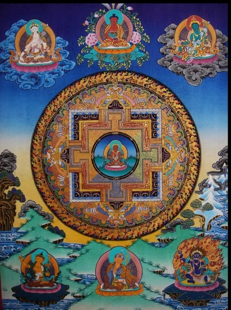
\includegraphics[scale=1]{cosmohindoue.png}
  \hspace{3cm}
  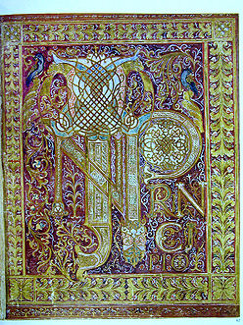
\includegraphics[scale=1]{genese.png}
  \caption{Gauche : illustration artistique de la cosmologie hindoue. Droite : couverture du livre de la Genèse, Bible de Staint-Paul-hors-des-Murs, vers 870.}
  \label{fig:cosmohindoue}
\end{figure}

Nous pourrions passer la totalité de ce manuscrit à décrire diverses cosmogonies. Mais celle qui nous intéresse et que nous allons détailler ici est la cosmogonie scientifique : la \emph{cosmologie}. La cosmologie est donc l'étude de l'univers, son origine, ses constituants et son devenir, dans le cadre de la méthode scientifique. Même si aujourd'hui la cosmologie fait consensus au sein des scientifiques en ce qui concerne la compréhension de l'univers, cela n'a pas toujours été le cas. Pendant longtemps les croyances religieuses ont dominé, allant jusqu'à limiter voire interdir les avancées scientifiques.
Il faut attendre le \textsc{XVI}\ieme~siècle pour que Copernic propose le modèle héliocentrique, soit presque \num{2000} ans après le modèle géocentrique d'Aristote, soutenu par l'église et les savants jusqu'alors.
% et s'oppose ainsi au modèle géocentrique introduit par d'Aristote et soutenu par l'église et les savants de l'époque.
Par la suite, les observations de Galilée, les travaux de Kepler ainsi que l'émancipation des dogmes religieux ont permis au modèle héliocentrique, fondé sur les lois de Kepler, de s'imposer. Cela a aussi permis à Newton de proposer sa théorie de la gravitation peu de temps après. Cette période marque la naissance de la physique et de la cosmologie.

Jusqu'au \textsc{XIX}\ieme~siècle, le modèle héliocentrique décrivant l'univers comme se limitant à notre système solaire fait consensus. Puis émerge l'idée que les étoiles sont d'autres systèmes solaires, notament grâce aux premières mesures de distance d'étoiles proches\footnote{Par exemple la mesure de la distance de 61 Cygni par Bessel en 1838. \#prov https://www.universalis.fr/encyclopedie/premiere-determination-de-la-distance-d-une-etoile/}. L'idée de galaxie, un système rassemblant une multitude de systèmes solaires, fait aussi sont apparition, nous conduisant vers un paradigme de moins en moins anthropocentrique.

\paragraph{}
La cosmologie moderne naît réellement au début du \textsc{XX}\ieme~siècle. En 1915, Einstein propose sa théorie de la gravitation : la \emph{relativité générale}. Elle offre une vision radicalement différente de la théorie bien établie de Newton. La gravitation n'est plus vue comme une force instantannée entre les corps massifs mais comme une déformation de l'espace temps se propageant à la vitesse de la lumière. La théorie d'Einstein explique avec succès l'avance du périhélie de Mercure, jusque là incompris. Puis en 1919 lors d'une éclipse de Soleil, la déviation de la lumière par un corps massif, prédiction directe de la relativité générale et non présente dans la théorie de Newton, est observée. \textbf{Non seulement la déviation de la lumière est observée pour la première fois, mais l'angle de déviation observé correspond à celui prédit par la théorie.}. Ceci assoit au sein de la communauté scientifique la théorie d'Einstein en tant que nouvelle théorie de la gravitation.

Par ailleurs, la cosmologie observationnelle connaît des avancées remarquables, notament grâce à Edwin Hubble qui observe le décalage vers le rouge\footnote{voir explication du redshift section \#prov:ref} du spectre d'objets lointains, dû à leur vitesse d'éloignement. Il comprend aussi que les objets étendus, jusque là interpretés comme des nuages de poussière et de gas et appelés nébuleuses, sont d'autres galaxies semblables à la nôtre. Parallèlement, Alexandre Friedmann résout en 1922 les équations d'Einstein de la relativité générale pour un univers homogène et isotrope et trouve une solution d'univers en expansion, qui contraste avec l'idée d'un univers statique et éternel jusque là ancrée dans les esprits. Enfin, Georges Lemaître effectue le lien entre tous ces éléments. En 1927, il publie un papier explicant que l'éloignement des galaxies et le décalage vers le rouge de leur spectre pouvait être expliqué par une théorie d'univers en expension, et donne la première estimation de la constante de Hubble\footnote{Constante reliant proportionnellement la vitesse d'éloignement des galaxies à leur distance, voir \#prov:ref}. En 1929, Edwin Hubble publie son célèbre papier, exposant la loi de Hubble et favorisant très fortement le modèle d'univers en expansion.

Nous pouvons noter ici que peu de temps après avoir publié sa théorie, Einstein ajoute dans ses équations une constante ad hoc, dite \emph{constante cosmologique}, et noté $\Lambda$. Cette constante est rajoutée afin de rendre les solutions à ses équations capables de décrire un univers statique (idée dominante de l'époque). Puis, suite à la publication de Hubble, Einstein retire la constante cosmologique de ses équations et la qualifie de ``plus grande bêtise de sa vie''. L'ironie fait qu'en 1998, la constante cosmologique est réintroduite dans les modèles afin d'expliquer l'observation de l'accélération de l'expansion de l'univers (voir \#prov ref). Les mesures les plus récentes estiment que la densité d'énergie de cette constante cosmologique, aussi appellée énergie sombre, représente environ \SI{70}{\percent} de l'énergie totale de notre univers.

\paragraph{}
Ces quinze années très fertiles pour la cosmologie ont popularisé l'idée d'un univers en expansion. Si certains s'y opposent et défendent un univers statique, d'autres s'y intéressent et étudient en détail les conséquences de ces modèles théoriques. Si l'univers est en expansion, c'est qu'il a été dans le passé plus petit qu'il ne l'est aujourd'hui. L'étude des solutions aux équations d'Einstein montre que l'expansion dilue la matière dans l'univers, et conduit à son refroidissement. L'univers était donc plus chaud et plus dense dans le passé. Si l'on remonte suffisament dans l'histoire de l'univers, celui ci devient de plus en plus petit, jusqu'à n'être à l'origine qu'un point infiniment chaud et dense. Ceci conduit à nommer ces classes de modèles \emph{hot big bang models}, ou modèles de big bang chaud en français.  \textbf{Il est à noter que cet \emph{instant zéro} est une extrapolation des modèles et reste hypothétique : au delà d'une certaine température, l'univers est tellement petit que les effets quantiques ne peuvent plus être négligés, rendant alors impossible l'utilisation de la relativité générale seule. Cet instant est appelé mur de Planck}. Afin de comprendre ce qu'il se passe entre le mur de Planck et l'instant zéro, une théorie traitant à la fois la gravitation et l'aspect quantique de la matière est nécessaire. C'est un domaine de recherche très dynamique aujourd'hui, dans lequel un grand nombre de théories de gravité quantique sont étudiées.
% . Ces points conduisent à nommer ces classes de solutions \emph{hot big bang models}, ou modèles de big bang en français, symbolisant l'idée qu'à l'origine\footnote{\#prov ou plutôt aussi loin que nous puissions remonter ? Ca vaut peut-être le coup d'expliquer la distinction}, l'univers fût un point infiniment chaud et dense.

Suite notament aux publications de Friedmann, Lemaître et Hubble, les défenseurs des modèles de big bang ont commencé à chercher des observables capables de prouver ces modèles. En 1948, George Gamow, Ralph Alpher et Robert Herman, reprenant les travaux de Georges Lemaître, prédisent l'existence du \emph{fond diffus cosmologique} (CMB : Cosmic Microwave Background). Ce rayonnement fossile, si les modèles de big bang sont vérifiés, aurait été émis lorsque l'univers était encore dense et chaud. Il repose sur l'idée que, du fait de la température initialement très élevée, les particules possèdent trop d'énergie pour s'assembler et former les premières briques élémentaires. L'univers n'est alors qu'une soupe où toutes les particules s'entrechoquent constamment. Lorsque l'univers s'expand, la température baisse et l'énergie des particules aussi, autorisant ainsi la formation des premiers noyaux d'atomes. Mais la température et la densité sont toujours trop importantes pour laisser les premiers atomes se former : l'univers est alors un bain de noyaux, principalement d'hydrogène et d'hélium, d'électrons et de photons. Les photons sont diffusés constamment sur les électrons libres, rendant le plasma de l'univers primordial opaque. Puis, lorsque l'univers devient suffisamment froid, les électrons ne disposant plus de suffisamment d'énergie sont capturés par les noyaux, formant les premiers atomes de l'univers. Ces atomes, neutres, ne diffusent pas les photons. Ces derniers peuvent alors se propager librement, et l'univers devient transparent. Ce sont ces premiers photons, émis environ \num{380000} ans après le big bang, qui forment le fond diffus cosmologique et que nous pouvons mesurer aujourd'hui. Les principales étapes sont résumées sur la figure~\ref{fig:univershistory}, dont notament la formation des premiers noyaux vers 0,01 seconde, puis le CMB vers \num{380000} ans.
En 1965, 17 ans après sa prédiction, le CMB est détecté par Penzias et Wilson, établissant ainsi le consensus sur les modèles de big bang. A partir de ce moment là, un certain nombre d'observations ont été menées par les cosmologistes afin de contraindre et distinguer les différents modèles de big bang.
\begin{figure}
  \centering
  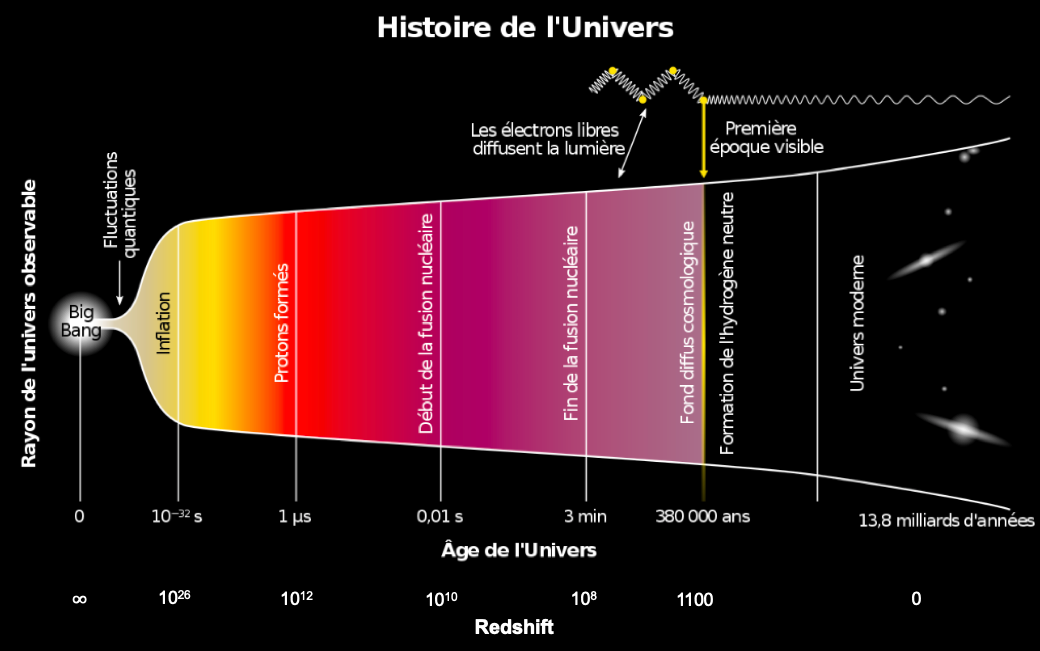
\includegraphics[scale=0.35]{univershistory2}
  \caption{Illustration de l'histoire de l'univers depuis ses origines jusqu'à aujourd'hui. Les principales étapes sont représentées : la formation des premiers protons et neutrons, puis des premiers atomes, et enfin l'emission du CMB. \#prov:rajouter la température, l'énergie, le redshift?}
  \label{fig:univershistory}
\end{figure}


\section{Le modèle \lcdm{}}

Le modèle \lcdm{} est aujourd'hui le modèle cosmologique qui fait consensus dans la communauté scientifique. Il est souvent désigné comme le modèle standard de la cosmologie. C'est un modèle de big bang, décrivant un univers composé principalement d'énergie noire, ou aussi appelé constante cosmologique ($\Lambda$), et de matière noire froide (CDM : Cold Dark Matter). La figure~\ref{fig:lcdm} présente la répartition de ses différents composants.
\begin{figure}
  \centering
  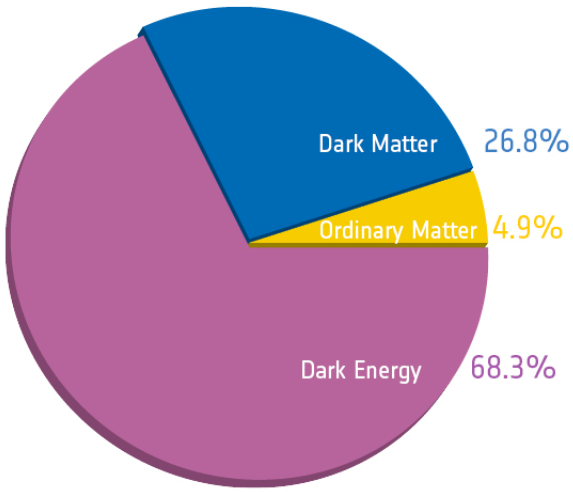
\includegraphics[scale=0.3]{lcdm}
  \caption{Répartition des différents composants du modèle \lcdm{}.}
  \label{fig:lcdm}
\end{figure}

Le modèle s'est établi suite à un certain nombre d'observations. D'abord, la détection du CMB en 1965, qui confirme les modèles de big bang.
Puis l'introduction de la matière noire dans les modèles au cours des années 70 et 80, notament grâce aux travaux de Vera Rubin sur le problème de la masse manquante dans les galaxies. Déja en 1933, Fritz Zwicky remarquait que la masse visible dans les amas n'était pas suffisante pour expliquer leur cohésion, et supposa donc l'existence d'une matière invisible. Une série d'observations fut menée dans les années 70 afin d'étudier les courbes de vitesse des étoiles au sein des galaxies. Les étoiles situées en périphérie furent mesurées avec une vitesse plus importante qu'attendue. La conclusion fut similaire à celle de Zwicky : la présence de masse invisible dans les halos de galaxies permet d'expliquer ces courbes de rotation. Ainsi la matière noire froide fut introduite dans les modèles cosmologiques : environ \SI{25}{\percent} de la masse de l'univers est sous la forme d'une matière non standard\footnote{Non-décrite par le modèle standard de la physique des particules} intéragissant uniquement via la gravitation avec la matière ordinaire.

% Plus tard, le satelitte COBE fut envoyé dans l'espace afin de mesurer le spectre\footnote{voir explication \#prov:ref} du CMB.
Plus tard, le satelitte COBE fut envoyé dans l'espace afin de détecter les anisotropies du CMB. Selon les prédictions des modèles de big bang, le spectre du CMB suit une loi de corps noir, avec une température d'environ \SI{3}{\kelvin}, et possède des anisotropies correspondant aux perturbations primordiales de densité. \textbf{La mission fut un succès : les mesures de COBE ont permis d'identifier les anisotropies de température du CMB, mettant en évidence les fluctuations de densité de l'univers primordial. D'autre part, le spectre du CMB est mesuré avec une température $T = \SI{2,73(6)}{\kelvin}$, ne déviant pas du spectre du corps noir de plus de \SI{0,25}{\percent} \cite{CITE:https://www.ncbi.nlm.nih.gov/pmc/articles/PMC46596/}. La détection des anisotropies du CMB constitue un des arguments les plus solides en faveur des modèles de big bang.}

Jusqu'alors, les modèles cosmologiques n'incluaient pas d'énergie noire. Puis en 1998, deux équipes différentes publient l'analyse de distances de luminosité de supernovae de type 1a (SN1a), toutes les deux mettant en évidence l'accélération de l'expansion de l'univers et donc favorisant les modèles contenant de l'énergie noire. Ce sont ces dernières observations qui ancrent \lcdm{} comme modèle de big bang préféré. Par la suite, le satellites WMAP puis le satellite Planck sont lancés en 2001 et en 2009 afin de mesurer avec une plus grande précision les anisotropies du CMB. Ces mesures successives sont effectuées avec une précision sans précédent, permettant de contraindre très fortement les paramètres cosmologiques. Les résultats finaux de la collaboration Planck ont été publiés en 2018~\cite{CITE:planck2018} et fournissent les paramètres cosmologiques du modèle \lcdm{} avec une précision inférieur au pourcent (\#prov:Ca vaut le coup de mettre le tableau qui résume les parametres cosmo?).

\subsection{Description du modèle}

Le modèle \lcdm{}, et plus généralement les modèles de big bang, sont fondés sur le formalisme de la relativité générale. \textbf{Cette théorie, élaborée par Einstein en 1915, fait deux postulats. D'abord, elle suppose l'unification de la masse et de l'énergie, via la célèbre formule\footnote{où $E$ est l'énergie, $m$ la masse, et $c$ la vitesse de la lumière dans le vide} $E = mc²$, ainsi que celle de l'espace et du temps. Ceci revient à se placer dans le cadre de la relativité restreinte. Elle suppose ensuite le principe d'équivalence}. Ce principe affirme que la masse inertielle et la masse gravifique sont équivalentes, et que les effets de la gravitation sont identiques aux effets de l'accélération du référentiel de l'observateur. Autrement dit, il n'existe pas d'expérience permettant à l'observateur de distinguer s'il se trouve dans un champ de gravitation ou dans un référentiel uniformément accéléré.

\paragraph{La métrique —}
\textbf{Le formalisme de la relativité générale s'appuie sur celui de la relativité restreinte. L'espace-temps est décrit par la métrique. Cet objet mathématique\footnote{Un tenseur de rang 2} permet de définir le produit scalaire sur l'espace-temps à 4 dimensions, et donc de mesurer les distances et les angles. C'est la métrique qui contient l'information sur la gravitation}. Dans le cadre du modèle \lcdm{}, la métrique utilisée est la métrique FLRW (pour Friedmann Lemaître Robertson Walker), elle s'exprime comme :
\begin{equation}
  \label{eq:metrique1}
  ds² = - c² dt² + R(t) \left[ \frac{dr²}{1 - k r²} + r² d\Omega \right],
\end{equation}
où $d\Omega = d\theta + \sin(\theta) d\phi$ , $R(t)$ rend compte de l'expansion de l'univers à l'instant $t$, et $k$ vaut soit $1$, $0$ ou $-1$ selon si l'univers possède une courbure positive, nulle ou négative (voir figure~\ref{fig:curvature}).
\begin{figure}
  \centering
  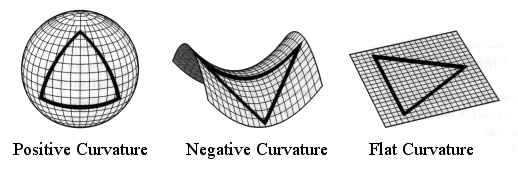
\includegraphics[scale=0.6]{curvature}
  \caption{Représentation de la courbure de l'univers : positive à gauche, négative au centre et nulle à droite. Crédits : http://abyss.uoregon.edu/~js/cosmo/lectures/lec15.html}
  \label{fig:curvature}
\end{figure}
A l'aide d'un changement de coordonnées, il est possible de se ramener à la formule suivante :
\begin{equation}
  \label{eq:metrique2}
  ds² = - c² dt² + a(t)\left[ d\chi² + S_{k}²(\chi) d\Omega \right],
\end{equation}
où $a(t) = R(t) / R(t₀)$,  $t₀$ est le temps présent et $S_{k}$ est défini comme
\begin{align}
  S_{k}(\chi) = R(t₀) \left\{
    \begin{array}{ll}
      sin(\chi / R(t₀)) & \mbox{si } k = 1 \\
      \chi / R(t₀) & \textrm{si } k = 0 \\
      sinh(\chi / R(t₀)) & \mbox{si } k = -1
    \end{array}
\right..
\end{align}
Cette formulation permet de mettre en évidence le rapport $a(t)$, appelé facteur d'échelle. Par définition il vaut 1 aujourd'hui. Afin de rendre compte de l'expansion, $a(t) < 1$ pour $t < t₀$ (passé) et $a(t) > 1$ pour $t > t₀$ (futur).

\paragraph{Le redshift —}
% Le décalage vers le rouge, ou \emph{redshift} en anglais, est une conséquense de la relativité générale. Les objets distants s'éloignent de nous du fait de l'expansion de l'univers. Similairement à l'effet Doppler\footnote{L'effet Doppler est l'augmentation ou la diminution de la longueur d'onde d'une onde lorsque l'émetteur de cette dernière s'approche ou s'éloigne de l'observateur. L'exemple le plus connu est celui de l'ambulance : le son entendu est plus aigu lorsque l'ambulance s'approche, puis plus grave lorsqu'elle s'éloigne.}, le spectre observé de ces objets est décalé vers les grandes longueurs d'onde. Mais contrairement à l'effet Doppler, le redshift n'est pas directement dû à la vitesse de recession de l'objet : les photons, lorsqu'ils se propagent de l'objet émetteur jusqu'à nous, subissent la dilatation de l'espace et perdent ainsi de l'énergie, leur longueur d'onde se trouvant augmentée \#correction: un peu fishy: demander a Jim sinon. Le redshift est donc du à l'expansion de l'univers. Il est d'ailleurs parfois nommé redshift cosmologique.
% Le redshift, noté $z$, est défini via la relation
% \begin{equation}
%   \label{eq:redshift}
%   1 + z = \frac{\lambda_{o}}{\lambda_{e}},
% \end{equation}
% où $\lambda_{e}$ est la longueur d'onde émise, et $\lambda_{o}$ la longueur d'onde observée. On peut montrer que le reshift est relié au facteur d'échelle via la formule
% \begin{equation}
%   \label{eq:redshift2}
%   1 + z = \frac{1}{a(t)}.
% \end{equation}
Le décalage vers le rouge, ou \emph{redshift} en anglais, est une conséquense de la relativité générale. Les objets distants s'éloignent de nous du fait de l'expansion de l'univers. Similairement à l'effet Doppler\footnote{L'effet Doppler est l'augmentation ou la diminution de la longueur d'onde d'une onde lorsque l'émetteur de cette dernière s'approche ou s'éloigne de l'observateur. L'exemple le plus connu est celui de l'ambulance : le son entendu est plus aigu lorsque l'ambulance s'approche, puis plus grave lorsqu'elle s'éloigne.}, le spectre observé de ces objets est décalé vers les grandes longueurs d'onde. \textbf{Mais contrairement à l'effet Doppler, le redshift n'est pas directement dû à la vitesse de recession de l'objet : les photons, lorsqu'ils se propagent de l'objet émetteur jusqu'à nous, subissent la dilatation de l'espace et voient leur longueur d'onde augmenter. Ceci est dû au facteur d'échelle $a$ présent dans la métrique. En effet, on peut montrer que
\begin{equation}
  \frac{\lambda_o}{\lambda_e} = \frac{a(t_e)}{a(t_o)} ,
\end{equation}
où $t_e$ et $t_o$ sont les temps d'émission et d'observation du photon, $\lambda_{e}$  et $\lambda_{o}$ sa longueur d'onde lors de l'émission et de l'observation. Le redshift est alors définit comme 
\begin{equation}
  \label{eq:redshift}
  1 + z = \frac{1}{a(t)}.
\end{equation}
Le redshift est donc directement du à l'expansion de l'univers. Il est d'ailleurs parfois nommé redshift cosmologique. Il peut servir de mesure de temps (et aussi de distance, voir distances \#prov) : le spectre d'un objet avec un redshift $z=2$ est décalé vers le rouge d'un facteur 3. Il en découle que sa lumière observé aujourd'hui a été émise lorsque l'univers avait une taille 3 fois plus petite qu'aujourd'hui, soit il y a environ 12 milliards d'annéees.}

% leur longueur d'onde se trouvant augmentée \#correction: un peu fishy: demander a Jim sinon. Le redshift est donc du à l'expansion de l'univers. Il est d'ailleurs parfois nommé redshift cosmologique.
% Le redshift, noté $z$, est défini via la relation
% \begin{equation}
%   \label{eq:redshift}
%   1 + z = \frac{\lambda_{o}}{\lambda_{e}},
% \end{equation}
% où $\lambda_{e}$ est la longueur d'onde émise, et $\lambda_{o}$ la longueur d'onde observée. On peut montrer que le reshift est relié au facteur d'échelle via la formule
% \begin{equation}
%   \label{eq:redshift2}
%   1 + z = \frac{1}{a(t)}.
% \end{equation}

% Ainsi le redshift peut servir de mesure de temps (et aussi de distance, voir distances \#prov) : le spectre d'un objet avec un redshift $z=2$ est décalé vers le rouge d'un facteur 3. Il en découle que sa lumière observé aujourd'hui a été émise lorsque l'univers avait une taille 3 fois plus petite qu'aujourd'hui, soit il y a environ 12 milliards d'annéees.

\paragraph{Les équations d'Einstein —}
Lorsqu'Einstein publie sa théorie en 1915, la façon de présenter les équations d'Einstein, le coeur de la théorie, est différente de la façon de les présenter aujourd'hui. Nous nous proposons ici de suivre l'approche de la physique moderne, qui formule toutes les théories en termes d'un seul et même principe : le \emph{principe de moindre action}. Ce principe stipule que l'action mis en oeuvre lors de l'évolution d'un système entre deux instants est toujours extrémale\footnote{Elle est minimale dans la grande majorité des cas.}. L'action est une quantité caractérisant globalement un système, elle est définie comme
\begin{equation}
  \label{eq:action}
  \mathcal{S} = \int_{t₀}^{t₁} L dt,
\end{equation}
où $L$ est le lagrangien du système. En mécanique newtonienne, il est défini comme la différence de l'énergie cinétique et de l'énergie potentiel. En relativité générale, tout comme dans les théories de champs\footnote{Par exemple la théorie quantique des champs.}, le terme du lagrangien est représenté plutôt par une densité de lagrangien. Cette densité de lagrangien est alors intégrée sur l'espace-temps afin d'obtenir l'action. Dans le cas de la relativité générale, l'action est définie comme
\begin{equation}
  \label{eq:actionrg}
  \mathcal{S} = \int d⁴x \sqrt{-g} \frac{R}{4 \pi G} ,
\end{equation}
où $g$ est le déterminant de la métrique, $R$ le scalaire de Ricci, et $G$ la constante de Newton. Une fois l'action déterminé, sa minimisation conduit aux équations du mouvement du système. Dans notre cas, ce sont les équations d'Einstein :
\begin{equation}
  \label{eq:einstein}
  R_{\mu \nu} - \frac{1}{2} R g_{\mu \nu} + \Lambda g_{\mu \nu} = 8 \pi G T_{\mu \nu},
\end{equation}
où $g_{\mu \nu}$ est la métrique, $R_{\mu \nu}$ le tenseur de Ricci, $T_{\mu \nu}$ le tenseur énergie-impulsion, et $\Lambda$ la constante cosmologique. L'équation~\ref{eq:einstein} regroupe en réalité plusieurs équations. Les indices $\mu$ et $\nu$ varient de 0 à 3, 0 représentant la coordonnée temporelle et 1 à 3 les coordonnées spatiales. Il existe donc une équation par couple $(\mu, \nu)$, produisant 16 équations. Par des arguments de symétrie, ce nombre se réduit à 6 équations indépendantes, que l'on nomme les équations d'Einstein.

\paragraph{Les équations de Friedmann-Lemaître —}
Les équations d'Einstein forment un système d'équations hautement non linéaire, et de fait, difficile à résoudre. Afin de simplifier les équations et trouver des solutions, certaines hypothèses sont faites. Dans la plupart des modèles cosmologiques, l'univers est supposé homogène et isotrope à grande échelle. C'est le cas de la métrique FLRW (voir eq.~\ref{eq:metrique2}). Dans un tel cas, il est aisé de calculer le membre de gauche de l'équation~\ref{eq:einstein}. Ce calcul, que nous ne détaillerons pas ici, passe par la détermination des symboles de Christoffel et est très bien détaillé dans \cite{prov: Dodelson 2.1.2}. De plus, si nous considérons que l'univers est constitué d'un fluide parfait, le tenseur énergie impulsion prend la forme
\begin{equation}
  T_{\mu \nu} =
  \begin{pmatrix}
    -\rho & 0 & 0 & 0 \\
    0 & \mathcal{P} & 0 & 0\\
    0 & 0 & \mathcal{P} & 0\\
    0 & 0 & 0 & \mathcal{P}
  \end{pmatrix} ,
\end{equation}
où $\rho$ est la densité du fluide, et $\mathcal{P}$ est sa pression. Dans ces conditions, la partie temporelle de l'équation~\ref{eq:einstein} donne
\begin{equation}
  \label{eq:friedmann1}
  \left(\frac{\dot{a}}{a}\right)^2 = \frac{8 \pi G}{3}\rho + \frac{\Lambda}{3} - \frac{k}{a^2} 
\end{equation}
et la partie spatiale
\begin{equation}
  \label{eq:friedmann2}
  2 \frac{\ddot{a}}{a} + \left(\frac{\dot{a}}{a}\right)^2 = - 8 \pi G \mathcal{P} + \Lambda - \frac{k}{a^2} ,
\end{equation}
où le point désigne la dérivé temporelle. On définit alors le taux d'expansion $H$ comme $H(t) = \frac{\dot{a}(t)}{a(t)}$. Sa valeur actuelle, notée $H₀$, est appelée constante de Hubble. Elle relie proportionnellement la distance des galaxies à leur vitesse d'éloignement, via la loi de Hubble :
\begin{equation}
  \label{eq:hubble}
  V = H_0 \times D.
\end{equation}
$H_0$ est souvent donné comme $H_0 = 100 h\,\mathrm{km \cdot s^{-1} \cdot Mpc^{-1}}$, où $h$ est un paramètre sans dimension qui caractérise notre ignorance sur $H_0$. D'après les mesures les plus récentes~\cite{CITE planck + Riess ?}, $h$ varie entre $\num{0,67}$ et $\num{0,75}$. L'équation~\ref{eq:hubble} est nommée en l'honneur d'Edwin Hubble, après sa publication en 1929, même si Georges Lemaître fut le premier à saisir le lien entre distance et vitesse d'éloignement des galaxies et son implication concernant l'expansion de l'univers. Suite à cette brève parenthèse, retournons à nos deux équations. Il est courant de récrire ces équations en injectant $H(t)$, ainsi qu'en remplaçant la seconde par une combinaison linéaire des deux précédentes :
\begin{align}
  \label{eq:friedmann3}
  % \left\{
  %   \begin{array}{l}
  H^2 &= \frac{8 \pi G}{3} \rho + \frac{\Lambda}{3} - \frac{k}{a^2} ,\\
  \label{eq:friedmann4}
        %         - 2 \dot{H} - 3 H^2 = 8 \pi G P + \Lambda + \frac{k}{a^2}
  \frac{\ddot{a}}{a} &= - \frac{4 \pi G}{3} (\rho + 3 P) + \frac{\Lambda}{3} .
        %       \end{array}
  % \right..
\end{align}
Ces deux équations sont appelées les équations de Friedmann-Lemaître. Elles découlent directement des équations d'Einstein et permettent de relier les densités d'énergie des différents composants de l'univers au facteur d'échelle. Dans notre cas, nous avons choisi un univers représenté par un unique fluide parfait. Cependant nous pouvons noter que le membre de droite de l'équations~\ref{eq:friedmann3} contient 3 entités plutôt qu'une seule : le fluide parfait ainsi que la courbure et la constante cosmologique. Même si cela reste un choix d'écriture et ne relève d'aucun argument mathématique, il permet de mettre en évidence le fait que ces 2 entités peuvent être considérées comme composant énergétique de l'univers, avec leur propre densité d'énergie.


\paragraph{Évolution de l'univers —}
Les équations de Friedmann-Lemaître permettent, pour un fluide donné, de déterminer l'évolution de $\rho$ et $\mathcal{P}$ en fonction du facteur d'échelle. Afin d'obtenir leur évolution temporelle ainsi que celle du facteur d'échelle, il est nécessaire d'ajouter une équation. L'équation généralement choisie est l'équation d'état d'un fluide parfait, reliant sa pression à sa densité :
\begin{equation}
  \label{eq:etat}
  \mathcal{P} = w \rho .
\end{equation}
De plus, en utilisant la conservation\footnote{Cette équation est l'analogue en relativité générale de la conservation de l'énergie. Le point-virgule désigne la dérivé covariante.} du tenseur énergie-impulsion $T_{\mu \nu ; \mu} = 0$, nous obtenons la relation de conservation
\begin{equation}
  \label{eq:conservation}
  \dot{\rho} + 3 H (\rho + \mathcal{P}) = 0 .
\end{equation}
Cette équation n'est pas indépendante des deux équations de Friedmann-Lemaître et peut aussi être obtenue avec une combinaison linéaire de ces deux dernières. En intégrant cette équation et en utilisant l'équation d'état~\ref{eq:etat}, nous obtenons donc l'évolution de $\rho$ avec le facteur d'échelle
\begin{equation}
  \label{eq:rho_vs_a}
  \rho = \rho_0 a^{-3(1+w)} ,
\end{equation}
où $\rho_0$ est la densité aujourd'hui. Ainsi, l'évolution de la densité d'énergie de notre fluide dépendra principalement de son paramètre d'état $w$. Si nous injectons maintenant cette équation dans l'équation~\ref{eq:friedmann3}, nous obtenons
\begin{equation}
  \label{eq:H_evol}
  H = H_0 a^{-3 (1+w) / 2} ,
\end{equation}
ce qui nous donne finalement
\begin{equation}
  \label{eq:a_vs_t}
  a(t) \propto t^{\frac{2}{3(1+w)}} .
\end{equation}

Ce raisonnement s'étend à plusieurs fluides. Selon le fluide considéré, la valeur de $w$ est différente. Nous pouvons déjà distinguer la matière relativiste de la matière non relativiste. La matière non relativiste $(m)$ ou simplement matière, se compose de la matière baryonique\footnote{La matière dite ``ordinaire'', que nous côtoyons dans la vie de tous les jours.} $(b)$ et de la matière noire froide $(c)$. Elle est dite ``pressureless'' (sans pression) car elle possède un paramètre d'état nul : $w_m = 0$. Nous avons alors : $\rho_m \propto a^{-3}$. \\
Concernant la matière relativiste, aussi appelée radiation $(r)$, elle composée des photons $(\gamma)$ et des neutrinos relativistes $(\nu)$. Son paramètre d'état est $w_r = 1/3$, ce qui donne $\rho_r \propto a^{-4}$. Nous pouvons remarquer que la densité de matière diminue proportionnellement au volume de l'univers, par simple effet de dilution. La densité de radiation possède un facteur $1/a$ supplémentaire. Ce facteur provient du redshift des photons observés, et s'ajoute au $1/a^3$ de la dilution.
% dû à l'augmentation de la longueur d'onde des photons avec l'expansion (\#correction fishy, voir avec Jim).
Afin de travailler avec des quantités sans dimension et normalisées, il est courant d'introduire la densité critique $\rho_{crit} = 3 H_0^2 / 8 \pi G$. L'équation~\ref{eq:friedmann3} s'écrit alors
\begin{equation}
  \label{eq:friedmann5}
  \frac{H^2}{H_0^2} = \frac{\rho}{\rho_{crit}} ,
\end{equation}
$\rho$ représente alors la densité total d'énergie de l'univers. Chaque composant peut être mis sous la forme
\begin{equation}
  \label{eq:def_omgega}
  \frac{\rho_i}{\rho_{crit}} = \Omega_i a^{-3 (1+w)} , 
\end{equation}
où $\Omega_i$ est le ratio de la densité de l'espèce $i$ par la densité critique aujourd'hui. Nous pouvons alors récrire~\ref{eq:friedmann5} comme
\begin{equation}
  \label{eq:friedmann6}
  \frac{H^2}{H_0^2} = \sum_i \Omega_i a^{-3 (1+w)} ,
\end{equation}
où $i$ court sur toutes les espèces contribuantes à l'énergie totale de l'univers. Nous avons déjà présenté deux d'entre elles : $\Omega_m$ et $\Omega_r$. Comme mentionné plus tôt, la courbure et la constante cosmologique participent au bilan énergétique global et peuvent être mises sous la forme d'une densité d'énergie, en introduisant
\begin{equation}
  \label{eq:omega_lambda}
  \Omega_{k} = - \frac{k}{a^2 H^2} , \hspace{1cm} \textrm{et} \hspace{1cm} \Omega_{\Lambda} = \frac{\Lambda}{3 H^2} .
\end{equation}
Nous pouvons remarquer ici que $\Omega_{\Lambda}$ est indépendant de $a$, d'où son nom de constante cosmologique. Il en découle $w_{\Lambda} = -1$ : la constante cosmologique peut être interprétée comme un fluide de densité d'énergie constante et de pression négative. Nous verrons par la suite que sa domination dans le bilan énergétique de l'univers actuel est responsable de l'accélération de l'expansion (\#prov voir paragraphe?).
Enfin, en utilisant les deux définitions précédentes, nous obtenons l'évolution du taux d'expansion
\begin{equation}
  \label{eq:friedmann7}
  \frac{H^2}{H_0^2} = \Omega_m a^{-3} + \Omega_r a^{-4} + \Omega_k a^{-2} + \Omega_{\Lambda}.
\end{equation}
Il en découle que pour un univers plat, $\Omega_k = 0$ et donc $\Omega_m + \Omega_r + \Omega_{\Lambda} = 1$.

\paragraph{Les distances —}
Du fait de la géométrie particulière de l'univers, la notion de distance n'est pas si intuitive. Nous présentons ici les distances utilisées en cosmologie. Elles sont très bien décrites dans \cite{CITE: Hogg 1999}, et nous suivons d'ailleurs ses notations. Définissons premièrement la quantité
\begin{equation}
  \label{eq:dist_ez}
  E(z) = \frac{H(z)}{H_0} 
  = \sqrt{\Omega_m a^{-3} + \Omega_r a^{-4} + \Omega_k a^{-2} + \Omega_{\Lambda}} ,
\end{equation}
ainsi que la distance de Hubble
\begin{equation}
  \label{eq:dist_hubble}
  D_H = \frac{c}{H_0} .
\end{equation}
Nous pouvons alors définir les distances suivantes :
\begin{itemize}[label=$\bullet$]
\item la distance comobile : c'est la distance qui sépare 2 objets suivant le flow(\#prov flot ? écoulement ?) de Hubble. Deux objets à un redshift $z$ et séparés d'une distance physique $D$ possèdent une distance comobile $(1+z)D$. La distance comobile le long de la ligne de visé est définie comme
  \begin{equation}
    \label{eq:dist_como}
    D_{C} = D_H \int_0^z \frac{dz'}{E(z')} .
  \end{equation}
  Deux objets à un redshift $z$ et séparés par un angle $\delta \theta$ sur le ciel possèdent une distance comobile $\delta \theta D_M$. $D_M$ est la distance comobile transverse. 
  Dans le cas où l'univers n'est pas plat ($\Omega_k \neq 0$), la distance comobile transverse $D_M$  n'est pas la même que la distance comobile le long de la ligne de visée $D_{C}$ :
  \begin{equation}
    \label{eq:dist_como_trans}
    D_M = \left\{
      \begin{array}{ll}
        D_H \frac{1}{\sqrt{\Omega_k}} sin(\Omega_k D_C / D_H) & \mbox{si } \Omega_k < 0 \\
        D_C & \textrm{si } \Omega_k = 0 \\
        D_H \frac{1}{\sqrt{\Omega_k}} sinh(\Omega_k D_C / D_H) & \mbox{si } \Omega_k > 0
      \end{array}
    \right..
  \end{equation}
  
\item La distance de diamètre angulaire : c'est la distance reliée à la taille apparente d'un objet. Deux objets à un redshift $z$ et séparés par un angle $\delta \theta$ sur le ciel possèdent une distance physique $\delta \theta D_A$. $D_A$ est la distance de diamètre angulaire. Elle diffère de $D_M$ du fait qu'elle considère la distance physique et non comobile entre les deux objets. Elle est donc reliée à $D_M$ par
  \begin{equation}
    \label{eq:dist_ang}
    D_A = \frac{D_M}{1+z}.
  \end{equation}

\item la distance de luminosité : elle est définie via la relation qui exprime le flux d'une source lumineuse en fonction de sa luminosité
  \begin{equation}
    \label{eq:dist_lum}
    F = \frac{L}{4\pi D_L²} \hspace{0.5cm} \rightarrow \hspace{0.5cm} D_L = \sqrt{\frac{L}{4 \pi F}} .
  \end{equation}
  Elle est reliée à la distance comobile transverse via
  \begin{equation}
    D_L = (1+z) D_M = (1+z)² D_A ,
  \end{equation}
  le facteur (1+z) supplémetaire provenant du fait que les photons sont redshiftés à cause de l'expansion.
\end{itemize}
Dans ce manuscrit, les distances qui nous intéressent particulièrement sont $D_C$ et $D_A$. Nous y ferons appel dans la section \#prov ref.

\paragraph{Les paramètres du modèle —} 
Le modèle \lcdm{} est un modèle décrit par 6 paramètres. Ils sont mesurés par le satellite Planck~\cite{CITE ref} avec une précision d'environ 1~\% et sont résumés dans le tableau~\ref{table:planck2018}. Les 6 paramètres mesurés par Planck sont
\begin{itemize}
\item $\Omega_bh^2$, la densité de baryons multipliée par $h^2$
\item $\Omega_ch^2$, la densité de matière noire multipliée par $h^2$
\item $\theta_{MC}$, une approximation de $\theta_*$ : l'angle sur le ciel de l'échelle acoustique
\item $\tau$, la profondeur optique au moment de la réionisation
\item $A_s$, l'amplitude du spectre de puissance des fluctuations primordiales 
\item $n_s$, l'indice spectrale du spectre de puissance des fluctuations primordiales
\end{itemize}


\begin{table}[h]
  \centering
  \caption{Paramètres cosmologiques mesurés par le satellite Planck. La partie supérieure du tableau indique les six paramètres ajustés aux données. La partie inférieure donne d'autres paramètres déduits de ces six paramètres ajustés. Ces chiffres sont tirés de la table 1.1 de~\ref{CITE ref}}
  \label{table:planck2018}
  \begin{tabular}{lc}
    \toprule
    Parameters & Combined \\
    \midrule
    $\Omega_{\mathrm{b}}h^2$\dotfill & $0.02233\pm0.00015$ \\
    $\Omega_{\mathrm{c}}h^2$\dotfill & $0.1198\pm0.0012$ \\
    $100\theta_{\mathrm{MC}}$\dotfill & $1.04089\pm0.00031$ \\
    $\tau$\dotfill & $0.0540\pm0.0074$ \\
    $\ln(10^{10}A_\mathrm{s})$\dotfill & $3.043\pm0.014$ \\
    $n_\mathrm{s}$\dotfill & $0.9652\pm0.0042$ \\
    \midrule
    $\Omega_{\mathrm{m}} h^2$\dotfill & $ 0.1428\pm 0.0011 $ \\
    $H_0 \,[\si{\kilo\meter\per\second\per Mpc}]$\dotfill & $67.37\pm0.54$ \\
    $\Omega_{\mathrm{m}}$\dotfill & $0.3147\pm0.0074$ \\
    $\mathrm{Age}\, [\mathrm{Gyr}]$\dotfill  & $13.801\pm0.024$ \\
    $\sigma_8$\dotfill & $0.8101\pm0.0061$ \\
    $S_8\equiv \sigma_8 (\Omega_{\mathrm{m}}/0.3)^{0.5}$\dotfill & $0.830\pm0.013$ \\
    $z_{\mathrm{re}}$\dotfill & $7.64\pm0.74$ \\
    $100\theta_\ast$\dotfill & $1.04108\pm0.00031$ \\
    $r_{\mathrm{drag}} \,[{\rm Mpc}]$\dotfill & $147.18\pm0.29$ \\
    \bottomrule
  \end{tabular}
\end{table}

De ces 6 paramètres se déduisent les autres, notament les densités d'énergies aujourd'hui, dont nous venons de parler. Certains sont indiqués dans la seconde partie du tableau~\ref{table:planck2018}, dont notamment $r_{drag}$, la taille de l'horizon acoustique aujourd'hui, ou encore $\Omega_m$ la densité relative de matière aujourd'hui. Les paramètres cosmologiques utilisés pour la confection des simulations présentées dans ce manuscrit et par le code d'analyse \picca{} sont légèrement différents de ceux présentés dans le tableau~\ref{table:planck2018}. Les voici :
\begin{equation}
  \label{eq:par_cosmo}
  \Omega_M = \num{0.31457} \hspace{0.5cm} ; \hspace{0.5cm} \Omega_k = \num{0} \hspace{0.5cm} ; \hspace{0.5cm} \Omega_{\Lambda} = \num{0.68543} .
\end{equation}



\section{La fonction de corrélation de la matière}

Plus tôt, nous parlions du spectre de puissance des fluctuations primordiales sans avoir auparavant défini de quoi il s'agissait. Nous donnons ici une explication du spectre de puissance, et de son analogue, la fonction de corrélation, objet d'étude de ce manuscrit.

\subsection{Une analogie avec le son}

Prenons l'exemple d'un instrument de musique très simple : le diapason.
% Lorsqu'il est joué, le diapason produit une note fixe, caractéristique de l'instrument. Le signal sonore en fonction du temps, qui correspond à l'évolution de la pression de l'air en fonction du temps, est alors très proche d'une sinusoïde.
% Lorsqu'il est joué, le diapason produit un signal sonore, correspondant aux ondes de pression se propageant dans l'air, très proche d'une sinusoïde. La note produite correspond alors à une fréquence particulière, carractéristique de l'instrument. Ce passage, du signal temporel à la fréquence correspondante, correspond à la transformé de fourrier. Chaque signal peut etre decompose ...
Le diapason a la particularité de produire un signal sonore très proche d'une sinusoïde. Le son qu'il produit correspond alors à une note particulière, d'une fréquence donnéee, caractéristique de l'instrument. Par opposition au diapason, la corde de guitare par exemple, lorsqu'elle vibre, produit un son composé de plusieurs fréquences : la fréquence fondamentale, qui donne la hauteur de la note, et les fréquences harmoniques, des multiples de la fréquence fondamentale. Ces fréquences harmoniques participent à la richesse du son de l'instrument. L'outil mathématique permettant d'étudier ces phénomènes s'appelle la transformation de Fourier. La transformation de Fourier permet d'associer à un signal temporel, sa transformée de Fourier, un signal dans l'espace des fréquences.

Reprenons l'exemple du diapason. Comme dit précédemment, le signal sonore produit est très proche d'une sinusoïde. La figure~\ref{fig:example_tf} illustre la transformation de Fourier : à gauche se trouve le signal temporel, qui correspond au signal sonore, et à droite se trouve la transformée de Fourier de ce signal. Le cas du diapason se situerait plutôt sur la première ligne, tandis que le cas de la corde de guitare ressemblerait plutôt à la troisième : une somme de sinusoïdes de différentes fréquences, la fréquence la plus basse donnant la fréquence fondamentale. Dans notre cas, nous pouvons remarquer que le signal dans l'espace fréquentiel est relativement simple : il indique la répartition des différentes fréquences présentes dans le signal temporel.
\begin{figure}[h]
  \centering
  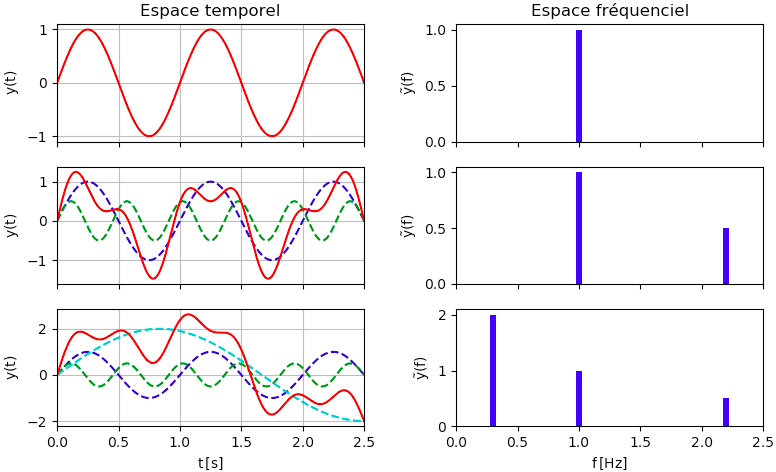
\includegraphics[scale=0.5]{example_tf}
  \caption{bla}
  \label{fig:example_tf}
\end{figure}

La transformation de Fourier permet donc de décomposer le signal temporel en une série de sinus et cosinus, et d'indiquer la répartition des différentes fréquences. Pour un signal temporel $F(t)$, la transformée de Fourier associée à ce signal est donnée par
\begin{equation}
  \label{eq:def_tf}
  \tilde f(\omega) = \frac{1}{\sqrt{2 \pi}} \int_{-\infty}^{+\infty}f(t) e^{-i \omega t} dt ,
\end{equation}
où $\omega$ est la pulsation. Elle est reliée à la fréquence $f$ par $\omega = 2 \pi f$.

\bibliographystyle{unsrt}
\bibliography{../source/biblio}

\end{document}
